\documentclass[10pt,a4paper]{article}
\usepackage{ucs}
\usepackage[utf8x]{inputenc}
\usepackage{amsmath}
\usepackage{amsfonts}
\usepackage{amssymb}
\usepackage[pdftex]{graphicx}

\usepackage[slovene]{babel}
\usepackage{lmodern}
\usepackage[T1]{fontenc}
\linespread{1.5}

\author{Vida Groznik, Anže Starič}
\title{Spomin}

\begin{document}
\maketitle
\newpage

\section{Uvod}
Spomin igra pomembno vlogo v našem življenju, saj predstavlja osnovo za učenje, sklepanje in razumevanje. Brez spomina bi dojemali le sedanjost in nebi mogli razumeti vzročnosti, saj bi do trenutka, ko bi videli rezultat neke akcije že pozabili, da smo akcijo izvedli.

Spomin v grobem delimo na eksplicitni (deklarativni) in implicitni (nedeklarativni) spomin. Kadar govorimo preprosto o spominu najpogosteje mislimo na {\bf eksplicitni spomin}. Do eksplicitnih spominov lahko dostopamo zavestno, enostavno jih tvorimo, ravno tako enostavno jih pozabljamo.

{\bf Implicitnega spomina} po drugi strani ne moremo uporabljati zavestno, vendar naučena opravila lahko opravljamo tudi brez zavestnega priklica (vožnja kolesa, prostoročno tipkanje, ...). Za tvorjenje implicitnih spominov potrebujemo več ponavljanja in vaje kot za tvorjenje eksplicitnih spominov, vendar jih zato težje pozabimo.

\section{Eksplicitni spomin}
Kot smo omenili v uvodu, eksplicitne spomine tvorimo in do njih dostopamo zavestno. Spominsko delovanje ločimo na pet procesov: {\it pozornost}, {\it vkodiranje}, {\it shranjevanje}, {\it konsolidacija} in {\it obnavljanje informacij}. {\it Pozornost} je sposobnost osredotočanja na določeno nalogo in igra pomembno vlogo pri izboru informacij, ki vstopajo v spominski proces. Drugi korak je {\it vkodiranje}, ki predstavlja registracijo informacij med procesom učenja. Če lahko informacijo povežemo z že znanimi asociacijami, je postopek vkodiranja bolj učinkovit. Ko je informacija vkodirana je {\it shranjena} v kratkoročni spomin. {\it Konsolidacija} je postopek organizacije kompleksnih informacij, pri katerem se prenesejo v dolgoročni spomin. Pri dostopanju do informacij gre za procese {\it obnavljanja informacij}, poznamo spontan priklic, priklic s pomočjo namiga in prepoznavanje. S priklicom in prepoznavanjem najlažje merimo sposobnost posameznikovega spominskega sistema.

Postopno pozabljanje je običajen proces našega spominskega sistema, kadar pa pride do večje izgube spomina, ki je posledica bolezni ali poškodbe govorimo o amneziji. Poznamo dve vrsti amnezije, {\it retrogradno amnezijo}, pri kateri gre za izgubo spominov pred poškodbo in {\it anterogradno amnezijo}, pri kateri gre za nezmožnost tvorjenja spominov po poškodbi. Bolnik, ki je doživel poškodbo pri 32 letih, katere posledica je bila retrogradna amnezija se tako ne more spomniti dgodkov, ki so se zgodili med njegovim 30 in 32 letom, če pa je posledica anterogradna amnezija, se ne more spomniti ničesar, kar se je zgodilo po njegovem 32 letu.

\subsection{Temporalni reženj}
\subsubsection{Bolnik H.M.}
Pri bolniku H.M so se okrog desetega leta začeli pojavljati epileptični napadi. Z leti so postajali vse hujši, vključevali so tresenje, grizenje jezika in izgubo zavesti. Ker zaradi epilepsije kljub jemanju zdravil ni mogel normalno delati, so mu pri 27 letih med operacijo izrezali dela obeh temporalnih režnjev. Od operacije dalje se pri bolniku epileptični napadi niso več pojavljali.

Odstranitev temporalnih režnjev ni vplivala na zavedanje, inteligenco ali osebnost bolnika H.M., vendar se je pri njem pojavila huda oblika amnezije. Opazni so bili znaki obeh vrst amnezije. Delna retrogradna amnezija se je kazala kot izguba spomina o dogodkih nekaj let pred operacijo, vendar je bolnik še vedno lahko priklical določene spomine iz otroštva. Anterogradna amnezija je bila prisotna v hujši obliki, zaradi nje bolnik ni prepoznal stvari, ki jih je spoznal nekaj minut nazaj. Bolnik si ni zapomnil niti zdravnice, ki je z njim delala vsak dan skoraj 50 let. Pri izvajanju preizkusa delovnega spomina (pomnjenje zaporedja števil) je bolnik dosegel običajen rezultat. V primeru, da je med izvajanjem poizkusa preusmeril pozornost na nekaj drugega, pa je poleg števil pozabil tudi, da si je moral zapomniti števila.

\begin{figure}[h]
  \centering
    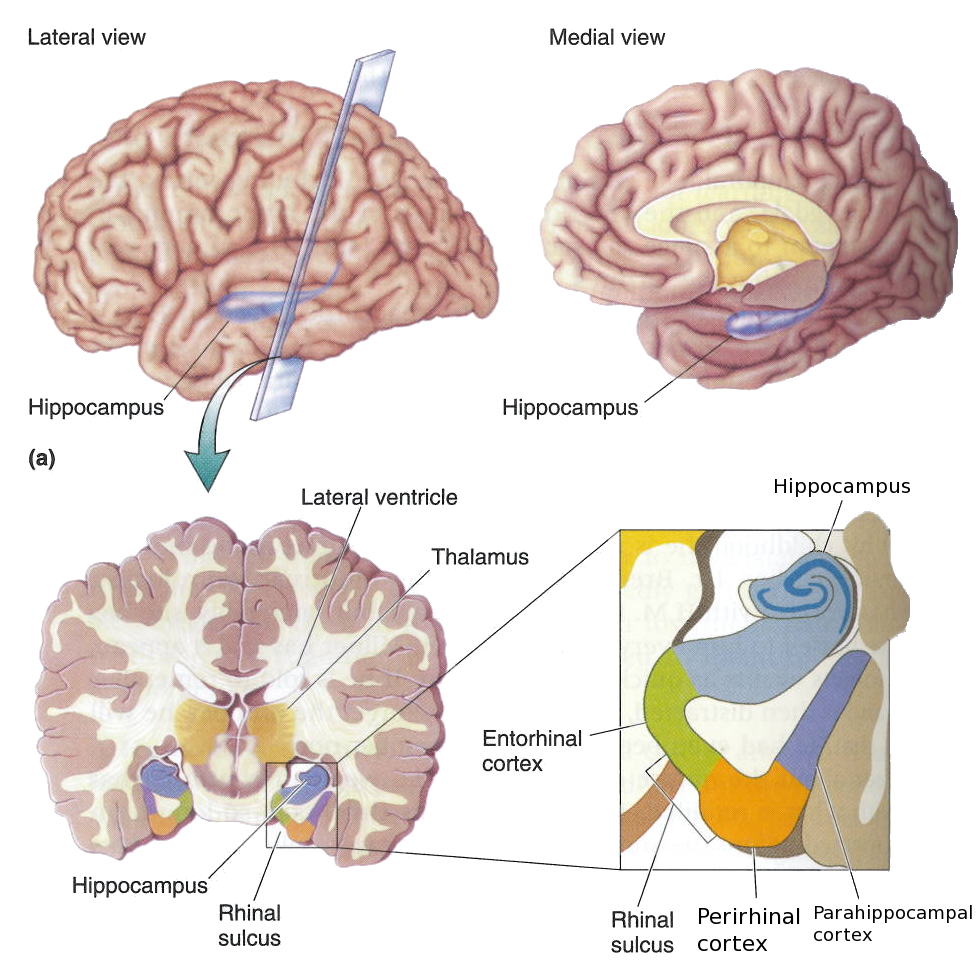
\includegraphics[width=1.0\textwidth]{LokacijaHippocampusa.png}
  \caption{Kje se nahaja hippocampus}
  \label{sHippocampus}
\end{figure}

\subsubsection{Vloga temporalnega režnja}
Iz primera bolnika H. M. lahko sklepamo, da po odstranitvi medialnih temporalnih režnjev dolgoročni in delovni spomin nista bila poškodovana, pojavila pa se je okvara sistemov za tvorjenje novih spominov. Pri operaciji so bili odstranjeni del hippocampusa, amygdala ter del korteksa (rhinalni sulcus in parahipocampalni cortex). Če opazujemo povezave v možganih opazimo, da vhod v medialni temporalni reženj prihaja iz asociacijskih področij. Informacije prehajajo preko korteksa do hippocampusa. V asociacijskih področjih se nahajajo močno obdelane informacije različnih modalnosti, kar pomeni, da vhod predstavljajo kompleksne predstavitve. Glavna izhodna povezava je {\it fornix}, ki gre mimo thalamusa in se konča v hypothalamusu.

Hippocampus skupaj z bližnjim korteksom sodeluje pri pretvarjanju informacij, ki prihajajo iz asociacijskih področij. Izgleda tudi, da strukture medialnih temporalnih režnjev sodelujejo pri konsolidaciji spominov. Hkraten pojav retrogradne in anterogradne amnezije pri bolnikih z okvaro medialnih temporalnih struktur namiguje tudi, da se v tem področju nekaj časa hranijo spomini, dokler se dokončno ne konsolidirajo v neokorteksu. Obstajajo še raziskave, ki kažejo, da hippocampus sodeluje pri obnavljanju informacij. To se odraža tako, da stimulacija pri določenih nevronih povzroči močnejši odziv, če je dražljaj poznan, kot če ni poznan. Pri drugih vrstah nevronov je odziv pri znanem dražljaju šibkejši, kot pri nepoznanem dražljaju. Iz dejstva, da pri znanem dražljaju pride do različnega odziva lahko sklepamo, da hippocampus sodeluje tudi pri priklicu spominov.

\subsection{Diencephalon}
\subsubsection{Bolnik N.A.}
N.A. je bil po poklicu vzdrževalec radarjev v ameriških zračnih silah. Nekega dne je sestavljal model letala, njegov cimer pa je za njegovim hrbtom vadil mečevanje. Ko se je N.A. v nepravem trenutku obrnil, se mu je meč skozi desno nosnico zapičil v možgane. Čez več let so ugotovili, da mu je pri te meč poškodoval le levi del thalamusa, ostali del možganov je bil nepoškodovan.

Po okrevanju se je kognitivna sposobnost vrnila na normalen nivo, vendar pa je imel težave s spominom. Imel je retrogradno amnezijo za obdobje dveh let pred nesrečo in precej hudo obliko anterogradne amnezije. Le-ta ni bila tako huda kot pri bolniku H.M, saj se je lahko spomnil nekaterih dogodkov in obrazov po nesreči, vendar so bili spomini površni. Čeprav je bila amnezija bolnika N.A. blažja, je po znakih zelo podobna amneziji bolnika H.M, delovni in dolgoročni spomin nista bila prizadeta, imel pa je težave s tvorjenjem novih spominov in retrogradno amnezijo, iz česar sklepamo, da tudi thalamus igra pomembno vlogo pri konsolidaciji spominov.

\section{Implicitni spomin}
\subsection{Proceduralni spomin}
Za proceduralni spomin bi v grobem lahko rekli, da je to spomin za opravljanje različnih nalog. Ko se pojavi potreba po opravljanju neke naloge, se avtomatsko prikliče in uporabi proceduralni spomin, ki vsebuje tako kognitivne kot tudi motorične spretnosti. Proceduralni spomin je vrsta dolgoročnega spomina, natančneje implicitnega spomina.

\subsubsection{Anatomska struktura}
\textbf{Striatum in bazalni gangliji}\\
Dorzolateralni striatum je povezan z učenjem navad in je glavno nevronsko celično jedro, ki je povezano s proceduralnim spominom. Povezovanje živčnih vlaken pomaga pri regulaciji aktivnosti v bazalnih ganglijih. Iz striatuma potujeta dve vzporedni poti za procesiranje informacij, ki delujate ena nasproti drugi pri kontroliranju gibanja in omogočata povezovanje z drugimi potrebnimi funkcionalnimi strukturami. Prva pot je neposredna, druga posredna in skupaj delujeta na tak način, da omogočata funkcionalne nevronske povratne zanke. Veliko povratnih povezav povezuje različne dele možganov s striatumom. Glavna povratna povezava, ki je povezana z motoričnimi spretnostmi, se imenuje korteks-bazalni gangliji-talamus-korteks zanka.

Dosedanje razumevanje možganske anatomije in fiziologije kažejo, da je stratumska zgradba tista, ki omogoča komunikacijo bazalnih ganglijev s strukturami in funkcionalno delovanje v procesiranju proceduralnega spomina. 
\\
\\
\textbf{Mali možgani}\\
Mali možgani so znani po tem, da igrajo ključno vlogo pri popravljanju gibanja in po piljenju proceduralnih motoričnih sposobnosti kot so slikanje, igranje instrumenta, in celo igranje golfa. Poškodbe tega dela lahko preprečijo ustrezno učenje motoričnih sposobnosti in s tem povezane raziskave so pokazale, da ima ta del vlogo pri avtomatiziranju nezavednih procesov pri učenju proceduralnih spretnosti.
\\
\\ 
\textbf{Limbični sistem}\\
Limbični sistem je skupina edinstvenih področij možganov, ki sodelujejo v številnih medsebojnih procesih, ki vključujejo čustva, motivacijo, učenje in spomin. TREnutna razmišljanja kažejo, da limbični sistem deli anatomijo z delom neostriatuma, ki je zaslužen za velike naloge nadzorovanja proceduralnega spomina. Ta vitalni del možganov najdemo na striatumovi zadnji meji in je bila šele pred kratkim povezana s spominom, sedaj pa jo imenujemo mejna delitev območja (MrD). Sledenje aktivacijam možganskih delov, ki sodelujejo med delovanjem proceduralnega spomina je možno zaradi proteinov v membrani limbičnega sistema.

\subsubsection{Testi}
Za testiranje delovanja spomina se uporablja več različnih testov.
\\
\\
\textbf{Zasledovanje premikanja}\\
Za preučevanje motoričnega učenja oseba z miškinim kurzorjem sledi premikajočemu objektu na ekranu. Tako izmerimo proceduralni spomin in pokažemo, koliko so izpiljeni gibi testirane osebe. Rezultati so prikazani kot razmerje med tem, koliko časa je oseba imela kurzor na objektu in koliko časa ne. Osebe z amnezijo ne kažejo oslabitve pri tem motoričnem testu pri nadaljnjih ponovitvah poizkusa. Vendar pa na to sposobnost vplivajo primankljaj spanca in uporaba drog.
\\
\\
\textbf{Merjenje reakcijskega časa}\\
Ta naloga vključuje, da sodelujoči ohranijo in se učijo proceduralnih sposobnosti, ki ocenjuje spomin za proceduralne motorične sposobnosti. Te sposobnosti se merijo z opazovanjem hitrosti in točnosti učenja ter ohranjanja novih sposobnosti. Reakcijski čas je čas, ki ga potrebuje udeleženec, da se odzove na dano iztočnico. Udeleženci z Alzheimerjevo boleznijo in amnezijo lahko dolgo časa hranijo naučeno sposobnost in lahko kasneje učinkovito opravijo takšno nalogo.
\\
\\
\textbf{Zrcalno sledenje}\\
Ta naloga se osredotoča na natančnejše povezovanje čutov, saj je to vizualno motorični test, kjer se morajo udeleženci naučiti nove motorične sposobnosti, ki vključuje koordinacijo rok in oči. Udeleženci z amnezijo so se sposobni naučiti in zapomniti to nalogo, kar nakazuje na proceduralni spomin. Risanje slike je namreč delo proceduralnega spomina; ko enkrat ugotovimo kako narisati podobo v zrcalu, imamo naslednjič s tem manj težav. Posamezniki z Alzheimerjevo boleznijo se ne morejo spomniti veščin, ki so jih pridobili v tej nalogi, vendar pa ne glede na uspešnost pridobijo proceduralno sposobnost.
\\
\\
\textbf{Naloga z napovedovanjem vremena}\\
Ta naloga uporablja eksperimentalno analizo napovedovanja vremena. To je naloga učenja verjetnosti v kateri mora udeleženec navesti, kakšno strategijo se uporablja za reševanje te naloge. Ta je orientirana kognitivno in se jo nauči na proceduralni način. Izvede se jo tako, da udeleženci dobijo set kartic z različnimi oblikami na podlagi katerih morajo napovedati izzid. Po podani napovedi udeleženci dobijo povratno informacijo in naredijo klasifikacijo na podlagi teh informacij. Udeleženci z amnezijo se med samim testiranjem te naloge naučijo, vendar se kasneje, ob ponovnem testiranju odrežejo precej slabše.


\subsubsection{Motnje}
Motnje so bile pomembne za razumevanje spominskega sistema. Sposobnosti spomina in zavore bolnikov z različnimi boleznimi so igrale pomembno vlogo pri ugotavljanju, da je dolgoročni spomin sestavljen iz različnih vrst spomina, natančneje iz deklarativnega in proceduralnega. Poleg tega so bili pomembni za osvetlitev strukture možganov, ki obsegajo nevronske mreže proceduralnega spomina.
Motnje, ki so pomagale pri razumevanju spomina so: 
\begin{itemize}
\item Alzheimerjeva bolezen in demenca
\item Sindrom Gilles de la tourete
\item Virus HIV
\item Huntingtonova bolezen
\item Obsesivna kompulzivna motnja (OCD)
\item Parkinsonova bolezen
\item Šizofrenija
\end{itemize}


\section{Delovni spomin}
Delovni spomin lahko testiramo z nalogo zakasnjenega priklica. Med tem ko opica opazuje položimo pod eno izmed dveh enakih posod hrano. Čez nekaj časa, med katerim opica ne vidi posod, ji dovolimo, da si izbere eno posodo. Poizkus je uspešen, če opica izbere posodo s hrano. Pri uspešnem izvajanju naloge ključno vlogo igra delovni spomin, saj mora opica v njem ohranjati informacijo, v kateri posodi je hrana.

Pri opicah z lezijami v prefrontalnem režnju uspešnost poskusa pada sorazmerno z naraščanjem časa, ko ne vidi posod iz česar lahko sklepamo, da je tudi prefrontalni reženj povezan s spominsko funkcijo možganov. Bolj zanimivo je opazovanje nevronov v prefrontalnem režnju. Če opazujemo aktivnost nevronov med izvajanjem naloge zakasnjenega priklica, lahko opazimo, da se nekateri nevroni prožijo ko opica opazuje postavljanje hrane ter ponovno ko opica izbira posodo. Drugi nevroni pa se prožijo med časom čakanja in prenehajo ko opica izbere posodo. Dejavnost teh nevronov ni direktno povezana z dražljajem, lahko pa sklepamo, da sodelujejo pri ohranjanju informacije v delovnem spominu.

\section{Poizkusi na podganah}
\subsection{Zvezdast labirint}
Večino stvari, ki jih vemo o spominu in delovanju hippocampusa smo izvedeli s pomočjo poskusov na podganah. Vloga hippocampusa pri podganah je bila razložena z uporabo \textbf{poskusa z zvezdastim labirintom}, prikazanem na sliki \ref{slikaLabirinta}. Pri tem poskusu na konec vsakega kraka postavimo košček hrane, nato pa v spomin spustimo podgano. Če v labirint spustimo normalno podgano, bo raziskovala labirint, dokler ne bo odkrila vseh koščkov hrane. Po večih poskusih se bo naučila nalogo opravljati učinkovito, tako da bo vsak krak labirinta obiskala le enkrat.

\begin{figure}[h]
  \centering
    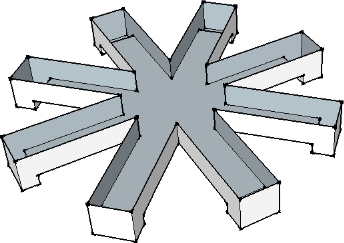
\includegraphics[width=.5\textwidth]{Labirint.png}
  \caption{Zvezdast labirint}
  \label{slikaLabirinta}
\end{figure}

Če v labirint spustimo podgano z uničenim hippocampusom, bo ravno tako raziskovala in se sčasoma naučila, da prehodi celoten krak in poje hrano na koncu, vendar se nikoli ne nauči učinkovitega opravljanja naloge. Taka podgana se bo večkrat vračala v že obiskane krake in zelo dolgo pustila nekatere krake s hrano ne obiskane. To lahko razložimo tako, da pojmujemo obiskovanje krakov in uživanje hrane na koncu kot dejanje, katerega se podgana nauči implicitno, izbor naslednjega kraka pa kot dejavnost, pri katerimi potrebujemo eksplicitni spomin o tem, katere krake smo že obiskali. Podgana z uničenim hippocampusom ima ovirano delovanje kratkoročnega spomina, zato se ne more naučiti optimalne strategije obiskovanja krakov. Dognanja se skladajo z ugotovitvami o človeškem hippocampusu.

Del poizkusa sva izvedla tudi sama. Pri poizkusu sva v labirintu testirala miši. Sprva so se prosto sprehajale po labirintu in se niso ozirale na hrano, pri naslednjih ponovitvah poskusa pa so se naučile, da se na koncih krakov nahaja hrana ter jih začele obiskovati. V petih ponovitvah poskusa se je ena od miši naučila pojesti ves sir v optimalnem obhodu (v noben krak ni vstopila dvakrat). Optimalni obhod je izvajala tudi pri nadaljnjih obhodih.

\subsection{Vodni labirint}
Številne raziskave dokazujejo, da je vsaj pri podganah hippocampus igra pomembno vlogo pri prostorskem spominu. Pri testiranju prostorskega spomina se uporablja \textbf{Morrisov vodni labirint}. V bazenu z mlečno vodo se nahaja dvignjena ploščad, preko katere lahko podgana spleza iz labirinta. Ko podgano prvič postavimo v labirint plava po njem, dokler ne naleti na ploščad in zleze nanjo. Pri nadaljnjih poskusih se podgana hitro nauči, kje se ploščad nahaja in plava naravnost proti njej. Podgane z omejenim delovanjem hippocampusa to nalogo slabše opravljajo.

\subsection{Prostorske celice}
Prostorske celice so odkrili, ko so z mikroelektrodami opazovali dejavnost hippocampusa pri podgani, ko se je premikala po škatli. Ko se je podgana seznanila s škatlo se je pojavila skupina nevronov, ki se je sprožila vsakič, ko je bila podgana v severozahodnem delu škatle. Od česa je odvisno proženje te skupine nevronov so testirali na dva načina. Pri prvem so vogale škatle označili s simboli. Po tem ko se je podgana seznanila s prostorom so jo umaknili ter obrnili škatlo za 180 stopinj. Ko so vrnili podgano vanjo so se prostorske celice prožile ob simbolu, ki je prej označeval severozahodni vogal in ne v severozahodnem vogalu. Pri drugem načinu testiranja so po tem, ko se je podgana seznanila s škatlo ugasnili luči. Prostorske celice so se še vedno prožile, čeprav podgana ni videla simbolov nad vogali. Iz tega lahko sklepamo, da prostorske celice označujejo, kje v prostoru podgana misli, da se nahaja.

\subsection{Relacijski spomin}
Posledica različnih poskusov na podganah je množica hipotez o aktivnostih, ki se dogajajo v hippocampusu. Eksperiment z vodnim labirintom in odkritje prostorskih celic nakazujeta, da je hippocampus zadolžen za prostorsko predstavo. Poizkus z zvezdastim labirintom pa, da hippocampus sodeluje pri uporabi kratkoročnega spomina. Hipoteza, ki povezuje obe odkritji trdi, da je hippocampus zadolžen za \textbf{relacijski spomin}. To pomeni, da sodeluje pri definiranju in hranjenju relacij med objekti.
\end{document}